\documentclass[11pt]{article}
\usepackage[portuguese]{babel}
\usepackage[utf8]{inputenc}
\usepackage[T1]{fontenc}
\usepackage{textcomp}
\usepackage{lmodern}
\usepackage{graphicx}

\setlength{\parskip}{2ex}
\def\aspa{\textquotesingle}

\setlength{\pdfpagewidth}{210truemm}
\setlength{\pdfpageheight}{297truemm}
\pdfadjustspacing=1

\topmargin -0.6in
\textheight 250truemm

\title{\vspace{8em} \huge{Wiki UFC} \\ \vspace{0.1em} \small{Especificação de Requisitos}}
\author{
	\vspace{5em} \\
	\small{Adriano Tavares} \\
	\small{Álinson Santos}  \\
	\small{André Castro}    \\
	\small{Luís Henrique}   \\
	\small{Rafael Barbosa}
}
\date{\today}

\begin{document}

\maketitle
\pagebreak

\tableofcontents
\pagebreak

\section{Introdução}
\subsection{Propósito do documento de requisitos}

O presente documento tem por objetivo mostrar uma descrição geral do produto, e, em seguida, especificar os requisitos de usuário e de sistema, funcionais e não funcionais. Sabendo do conjunto diversificado de usuários que podem ter acesso a este documento, procuramos utilizar uma linguagem de alto nível, embora, em certas ocasiões, o uso de alguns termos técnicos é necessário.

\subsection{Escopo do produto}

Sistema online colaborativo, na forma de wiki, onde os alunos poderão compartilhar informações sobre as disciplinas do curso. Cada disciplina terá uma página no Wiki; um repositório, onde os alunos poderão disponibilizar arquivos relacionados; um mural, para divulgação de notícias; e um calendário, que conterá datas de provas e trabalhos.

Sendo um sistema voltado para o aluno, não serão implementados sistemas de entrega de trabalhos, aulas e avaliações em tempo real, nem qualquer outro recurso semelhante encontrado em softwares de e-learning.

\subsection{Visão geral do restante do documento}

Em seguida, temos uma descrição mais detalhada do produto, incluindo seus requisitos.

Na seção 2, fornecemos uma descrição geral do sistema, contendo: descrição do produto (seção 2.1), de forma a melhor apresentar o contexto de aplicação em que se inserem os requisitos descritos no presente documento; e perfil do usuário (seção 2.2), esclarecendo a que tipo de usuário o sistema é destinado.

Na seção 3, é apresentada uma descrição dos requisitos, tanto funcionais (seção 3.2) quanto não funcionais (seção 3.3), além de diagramas de caso de uso (seção 3.1).

\section{Descrição Geral}
\subsection{Descrição do produto}

O Wiki UFC é uma aplicação com a finalidade de centralizar informações relacionadas às disciplinas do curso.

A idéia inicial do sistema surgiu quando se percebeu certas desvantagens do processo atual que os alunos utilizam para se comunicar. O material didático é muitas vezes segmentado em diferentes meios de comunicação e um esforço por parte do estudante é exigido para estar atualizado com a disciplina. O Wiki UFC tem o objetivo de diminuir este esforço, fornecendo um ambiente centralizado para compartilhamento de informações. Para cada disciplina, teremos:

\begin{itemize}
    \item Um espaço wiki
    \item Um mural para expor avisos
    \item Um calendário com os principais eventos da disciplina
    \item Um repositório para disponibilizar arquivos relacionados
\end{itemize}

\subsection{Perfil do usuário}

Sendo o sistema desenvolvido voltado para o gerenciamento de informações relacionadas às disciplinas acadêmicas, o público principal do sistema são estudantes, particularmente universitários.

\section{Requisitos específicos}
\subsection{Diagrama de Caso de Uso}
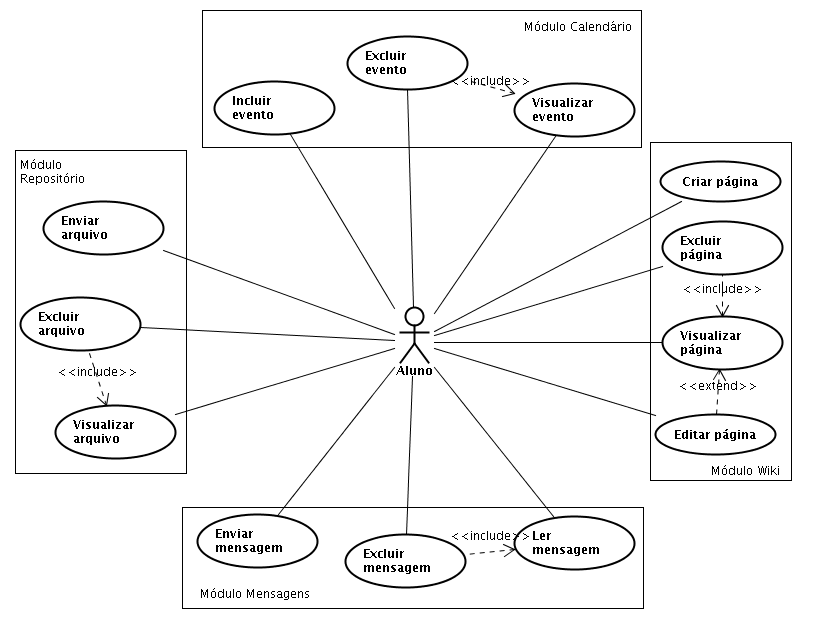
\includegraphics[width=1.20\textwidth]{usecase.png}

Cada caso de uso mostrado acima é melhor descrito na próxima seção do documento.

\subsection{Requisitos Funcionais}

\subsubsection{Módulo Wiki}
\textbf{Visualizar página}
\\

Nome:

      Visualizar página

Sumário:

      O usuário visualizará o conteúdo de uma página do wiki.

Ator Primário:

      Aluno. 

Fluxo Principal:

      Usuário navega até a página da disciplina na qual ele está interessado, consulta a lista de páginas wiki disponíveis, e clica sobre o título da página desejada. 

\textbf{Editar página}
\\

Nome:

      Editar página

Sumário:

      O usuário modificará o conteúdo de uma página do wiki. 

Ator Primário:

      Aluno. 

Fluxo Principal:

      Usuário navega até a página wiki desejada, e clica no link 'Editar'. Uma tela é exibida, onde o usuário poderá digitar o novo texto da página. O usuário então clica em 'Salvar'. 

Pós-Condições:

      A página wiki editada pelo usuário ficará com o novo texto digitado pelo usuário. A versão anterior estará disponível no link 'Histórico'. 

\textbf{Criar página}
\\

Nome:

      Criar página 

Sumário:

      O usuário criará uma nova página wiki. 

Ator Primário:

      Aluno. 

Fluxo Principal:

      O usuário navegará até a página da disciplina desejada e clicará no link correspondente à opção 'Nova Página'. Uma tela irá aparecer, e o usuário poderá digitar o conteúdo da nova página. Depois, o usuário clicará em 'Salvar'. 

Pós-Condições:

      A página recém criada será incorporada à lista de páginas wiki da disciplina, e poderá ser lida e editada por outros alunos. 

\textbf{Excluir página}
\\

Nome:

      Excluir página. 

Sumário:

      O usuário excluirá uma página do wiki. 

Ator Primário:

      Aluno. 

Fluxo Principal:

      O usuário navegará até a página wiki desejada, clicará em 'Editar' e, na nova tela que surgir, escolherá a opção 'Excluir página'. 

Pós-Condições:

      Após confirmar a exclusão, a página será excluída, e não será mais acessível a outros alunos. 

\subsubsection{Módulo Repositório}
\textbf{Visualizar arquivo}
\\

Nome:

      Visualizar arquivo. 

Sumário:

      O usuário visualizará o conteúdo de um arquivo do repositório. 

Ator Primário:

      Aluno. 

Fluxo Principal:

      O usuário navegará até a página da disciplina desejada, consultará a lista de arquivos disponíveis no repositório, e clicará sobre o arquivo que ele deseja visualizar. 

\textbf{Enviar arquivo}
\\

Nome:

      Enviar arquivo. 

Sumário:

      O usuário enviará um novo arquivo para a página da disciplina. 

Ator Primário:

      Aluno. 

Fluxo Principal:

      O usuário navegará até a página da disciplina desejada, clicará no link correspondente a 'Adicionar arquivo', selecionará o arquivo a ser enviado, e clicará no link 'Enviar'. 

Pós-Condições:

      O arquivo escolhido pelo usuário será enviado para o sistema, e poderá ser visualizado pelos demais alunos. 

\textbf{Excluir arquivo}
\\

Nome:

      Excluir arquivo. 

Sumário:

      O usuário excluirá um arquivo do repositório. 

Ator Primário:

      Aluno. 

Fluxo Principal:

      O usuário navegará até a página da disciplina e escolherá o link 'Excluir arquivo' correspondente ao arquivo que ele deseja excluir. 

Pós-Condições:

      O arquivo excluído não estará mais disponível para os demais alunos. 

\subsubsection{Módulo Calendário}
\textbf{Visualizar eventos}
\\

Nome:

      Visualizar eventos. 

Sumário:

      O usuário visualizará os eventos de um calendário. Poderá clicar em certo evento para obter maiores detalhes. 

Ator Primário:

      Aluno. 

Fluxo Principal:

      O usuário navegará até a página da disciplina desejada, onde poderá acessar o calendário da disciplina. 

\textbf{Incluir eventos}
\\

Nome:

      Incluir eventos. 

Sumário:

      O usuário incluirá novos eventos a um calendário de uma disciplina. 

Ator Primário:

      Aluno. 

Fluxo Principal:

      O usuário navegará até a página de calendário da disciplina e escolherá o link "Novo Evento", inserindo informações como título do evento, data e descrição. 

Pós-Condições:

      O evento inserido será adicionado à lista de eventos do calendário e poderá ser visualizado e poderá ser visualizado pelos demais alunos. 

\textbf{Excluir eventos}
\\

Nome:

      Excluir eventos. 

Sumário:

      O usuário excluirá eventos de um calendário de uma disciplina. 

Ator Primário:

      Aluno. 

Fluxo Principal:

      O usuário navegará até a página de calendário da disciplina e escolherá o link "Excluir Evento" associado ao evento que ele deseja excluir. 

Pós-Condições:

      O evento excluído será retirado da base de dados e não estará mais disposto para visualização pelos demais alunos. 

\subsubsection{Módulo Mensagens}
\textbf{Enviar mensagens para a Shoutbox}
\\

Nome:

      Enviar mensagens para a Shoutbox. 

Sumário:

      O usuário irá enviar uma mensagem por ele redigida para a Shoutbox. 

Ator Primário:

      Aluno. 

Fluxo Principal:

      O usuário, a partir de qualquer página no Wiki, digitará uma mensagem e a enviará para o Shoutbox. 

Pós-Condições:

      A mensagem enviada será mostrada na Shoutbox para os outros usuários autenticados no sistema no momento. 

\textbf{Enviar mensagens para o Mural}
\\

Nome:

      Enviar mensagens para a Mural. 

Sumário:

      O usuário irá enviar uma mensagem por ele redigida para o Mural. 

Ator Primário:

      Aluno. 

Fluxo Principal:

      O usuário, através do Mural de cada disciplina, digitará uma mensagem e a enviará. 

Pós-Condições:

      A mensagem será disponibilizada no Mural da disciplina, podendo ser vista por outros usuários que acessem a página da disciplina em questão. 

\textbf{Enviar mensagens para outros usuários}
\\

Nome:

      Enviar mensagens para outros usuários. 

Sumário:

      O usuário irá enviar uma mensagem por ele redigida para um outro usuário do sistema. 

Ator Primário:

      Aluno. 

Fluxo Principal:

      O usuário digitará uma mensagem, assinalará um destinatário, também usuário do sistema, e enviará a mensagem para este usuário assinalado. 

Pós-Condições:

      A mensagem será disponibilizada ao usuário destinatário, e somente a ele, podendo ser visualizada em sua página principal. 

\textbf{Ler mensagens}
\\

Nome:

      Ler mensagens. 

Sumário:

      O usuário irá ler uma mensagem, podendo ser esta redigida por ele mesmo ou por outro usuário. 

Ator Primário:

      Aluno. 

Fluxo Principal:

      O usuário entrará em alguma das seções que disponibilizam mensagens, e a interface do sistema formatará as mensagens arquivadas para serem visualizadas pelo usuário. 

Pós-Condições:

      Nenhuma. 

\textbf{Excluir mensagens}
\\

Nome:

      Excluir mensagens. 

Sumário:

      O usuário excluirá uma mensagem do sistema. 

Ator Primário:

      Aluno. 

Fluxo Principal:

      O usuário navegará até a seção onde está disponibilizada a mensagem e indicará a mensagem a ser apagada. 

Pós-Condições:

      A mensagem excluída não estará mais disponível para visualização pelos demais usuários. 



\subsection{Requisitos Não-Funcionais}

\subsubsection{Requisitos da Interface}

Dada a diversidade de alunos presentes na universidade, e os seus diferentes níveis de conhecimento técnico sobre a Internet, a interface do sistema precisa ser fácil de se utilizar.

\subsubsection{Restrições do Wiki}
\begin{itemize}
\item Detecção de Tags Maliciosas

Um conhecido tipo de falha de segurança em sistemas Web é o Cross-site scripting, abreviado XSS. Através de tags maliciosas inseridas no wiki, um usuário mal intencionado poderia comprometer a segurança do sistema, e expor os alunos a riscos. Assim, o wiki deve ser capaz de detectar e remover estas tags maliciosas.

\item Integridade dos Dados

Os dados fornecidos pelos usuários são de grande importância para a sobrevivência do sistema. Dessa forma, o wiki deve garantir que esses dados não sejam corrompidos. Ou seja, ele deve impedir que versões antigas da página sejam substituídas indevidamente.  
\end{itemize}

\end{document}
